\documentclass[hyperref=colorlinks]{beamer}
\mode<presentation>
\usetheme{iclpt}
\setbeamertemplate{navigation symbols}{}
\setbeamertemplate{headline}{
%\setbeamercolor{institute in head/foot}{fg=beamer@iclightblue,bg=beamer@icmiddleblue}
%% \begin{beamercolorbox}[leftskip=.05\textwidth,rightskip=.05\textwidth,ht=.07\textheight,dp=0.1cm,wd=\textwidth]{institute in head/foot}
%% \end{beamercolorbox}
}
\setbeamertemplate{footline}{
%%\begin{beamercolorbox}[ht=.1\textheight,dp=0.4cm,wd=\textwidth,leftskip=3cm]{author in head/foot}%
  %% \begin{minipage}[c]{5cm}%
%%     \usebeamerfont{author in head/foot}
%%   \end{minipage}\hfill%
%%   \hfill
%%   \begin{minipage}{6cm}
%%     \hfill
%%   \end{minipage}
%%\end{beamercolorbox}%
}

\usepackage{color}
\usepackage{tabularx,colortbl}
\usepackage{graphicx}
\usepackage{pdfpages}
\usepackage{feynmp}
\usepackage[orientation=landscape,size=a1,scale=1.3,debug]{beamerposter}
\DeclareGraphicsRule{*}{mps}{*}{}

\title{}
%\subtitle{AN-12-403,PAS-HIG-13-013 \vspace{-0.7cm}}
\author{P. Dunne, Imperial College London}%{ D.Colling, \underline{P. Dunne}, A. Magnan, A. Nikitenko, J. Pela with \\ R. Aggleton, J. Brooke: Bristol \\ C.Asawangtrakuldee, Q.Li: Peking \\ P. Srimanobhas: Chulalongkorn \\ S. Kumar, K. Mazumdar: Mumbai}
\date{}

\begin{document}
\begin{fmffile}{feynmandiags}
  
  \section{Title}
  \begin{frame}[t]
    \centering
    \vskip 1cm {\color{beamer@icdarkblue}\Huge VBF produced Higgs decays to invisible final states at CMS}
    
    \vspace{.5cm}    
    \centering
    \begin{columns}
      \column{.2\textwidth}
      
\includegraphics[height=.08\textheight]{icl.pdf} 
      \column{.6\textwidth}
      \centering
      \huge {\color{beamer@icmiddlered} Patrick Dunne, pdunne@cern.ch}
      \column{.2\textwidth}
      \hfill 
\includegraphics[height=.085\textheight]{../Pics/CMS-Color.pdf}
    \end{columns}

    \vspace{.5cm}

    \begin{columns}
      \column{.66\textwidth}%COLUMNS 1&2
      
      \begin{columns}
      \column{.49\textwidth}%COLUMN 1
      \begin{minipage}[t][.6\textheight][t]{\linewidth}
        \begin{block}{\LARGE Why VBF Higgs to invisible?}
          \begin{itemize}
            \vspace{.5cm}
          \item Many beyond the Standard Model theories predict significant invisible branching fractions, BF(inv), for the Higgs boson:
          \item[-] SUSY, extra dimensions, dark matter, etc.
            \vspace{.5cm}
          \item The only signature is the other particles produced with the Higgs, so associated production is necessary.
            \vspace{.5cm}
          \item Vector Boson Fusion (VBF) production's distinctive topology makes it the most promising channel:
          \item[-] the expected limit on BF(inv) is 53\% compared to 84\% (ATLAS) and 91\% (CMS) from ZH.
            \vspace{.5cm}
          \end{itemize}
          \centering
          %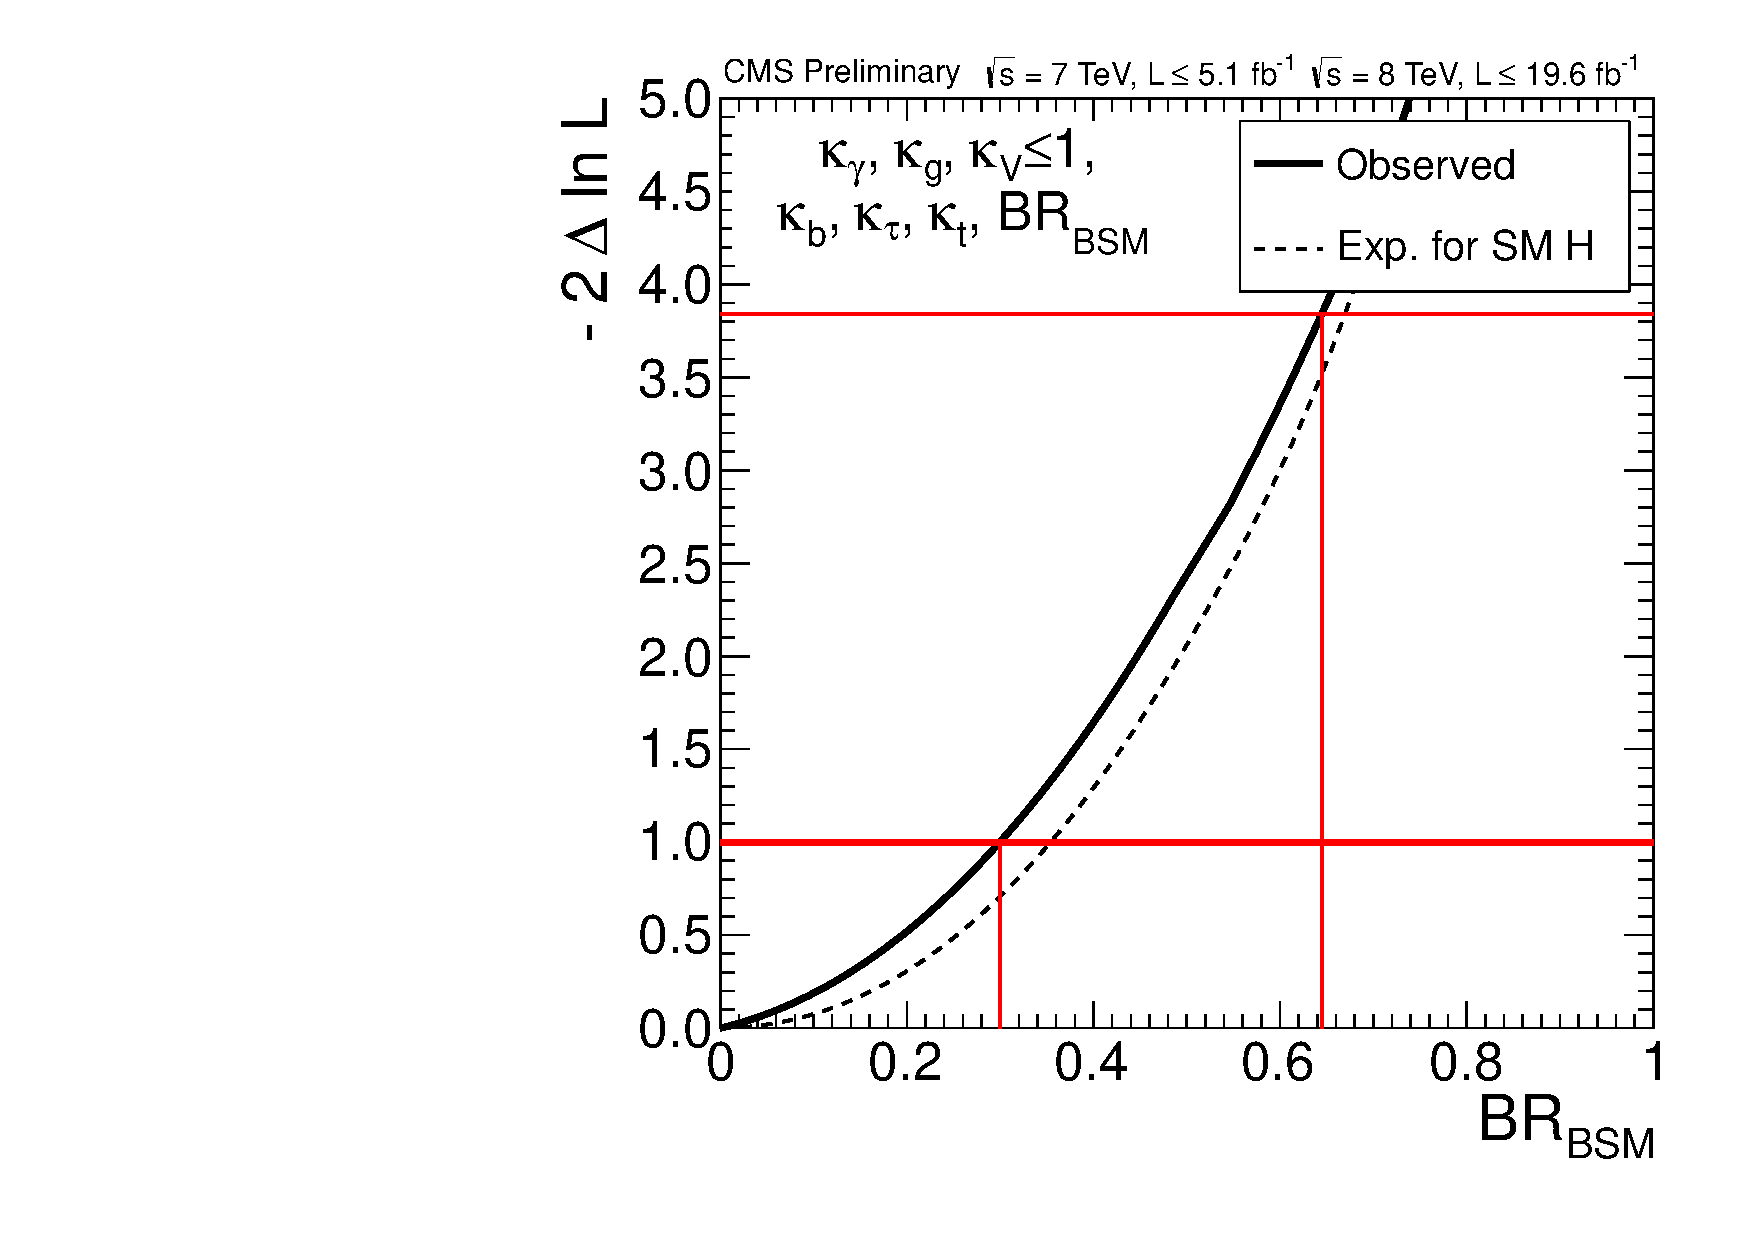
\includegraphics[width=.7\textwidth,height=.5\textwidth]{../invisible/TalkPics/invbr.pdf}
        
          \vspace{0.5cm}
        
        \end{block}
        

        \begin{block}{\LARGE Main backgrounds}
          %\vspace{.4cm}
          \begin{columns}
            \column{.6\textwidth}
            \begin{itemize}
              \vspace{.5cm}
            \item Leptonic $W$ + jets:
            \item[-] reduced by lepton veto,
            \item[-] remaining contribution where lepton is missed,
            \end{itemize}
            \column{.3\textwidth}
            %WJETS
            \hfill
            \begin{fmfgraph*}(150,120)
              \fmftop{i1,m1,m2,o1}
              \fmfbottom{i2,o2}
              \fmf{fermion,label=$e/\mu/\tau$,label.side=left}{v2,m1}
              \fmf{fermion,label=$\nu$,label.side=right}{v2,m2}
              \fmf{photon,tension=7/5,label=$W$}{v1,v2}
              \fmf{fermion}{v1,i2}
              \fmf{fermion}{v1,o2}
              \fmflabel{$jet$}{i2}
              \fmflabel{$jet$}{o2}
            \end{fmfgraph*}
            \column{.05\textwidth}
          \end{columns}

          \vspace{.25cm}
          
          \begin{columns}
            \column{.6\textwidth}
            \begin{itemize}
            \item $Z\rightarrow\nu\nu$ + jets:
            \item[-] irreducible.
            \end{itemize}
            \column{.3\textwidth}
            %ZJETS
            \hfill
            \begin{fmfgraph*}(150,100)
              \fmftop{i1,m1,m2,o1}
              \fmfbottom{i2,o2}
              \fmf{fermion}{v1,i2}
              \fmf{fermion}{v1,o2}
              \fmf{photon,tension=7/5,label=$Z$}{v1,v2}
              \fmf{fermion,label=$\nu$,label.side=left}{v2,m1}
              \fmf{fermion,label=$\nu$,label.side=right}{v2,m2}
              \fmflabel{$jet$}{i2}
              \fmflabel{$jet$}{o2}
            \end{fmfgraph*}
            \column{.05\textwidth}
          \end{columns}

          \vspace{.25cm}

          \begin{columns}
            \column{.6\textwidth}
            \begin{itemize}
            \item QCD multijets:
             \item[-] reduced by central jet veto and jet topology cuts.
             \end{itemize}
             \column{.3\textwidth}
             %QCD
             \hfill
             \begin{fmfgraph*}(150,120)
               \fmftop{i1,m1,m2,m3,m4,o1}
               \fmfbottom{i2,o2}
               \fmf{fermion,tension=4}{v1,i2}
               \fmf{fermion,tension=4}{v1,o2}
               \fmf{fermion,label=$jets$,label.side=left}{v1,m1}
               \fmf{fermion}{v1,m2}
               \fmf{fermion}{v1,m3}
               \fmf{fermion}{v1,m4}
               \fmflabel{$jet$}{i2}
               \fmflabel{$jet$}{o2}
             \end{fmfgraph*}
             \column{.05\textwidth}
           \end{columns}
           \vspace{.5cm}
         \end{block}

       \end{minipage}
       \column{.49\textwidth}%COLUMN 2
       \begin{minipage}[t][.6\textheight][t]{\linewidth}

         \begin{block}{}
           \centering
           \vspace{0.0225\textwidth}

           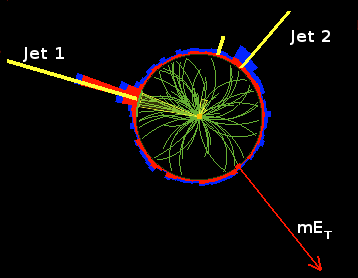
\includegraphics[width=.75\textwidth,trim=0 0 0 0]{Pictures/modifiedeventdisplay.png}

           \vspace{0.0225\textwidth}
         \end{block}


         \begin{block}{\LARGE Measurement strategy}
           \begin{itemize}
             \vspace{.5cm}
           \item Perform a counting experiment.
             \vspace{.5cm}
           \item Select distinctive VBF topology:
           \item[-] 2 jets with a large pseudorapidity separation,
           \item[-] veto events with central jets or any leptons.
             \vspace{.5cm}
           \item Require missing transverse energy, which is expected due to the invisible final state.
             \vspace{.5cm}
           \item Use hard cuts to restrict backgrounds.
             \vspace{.5cm}
           \item Use data driven methods to estimate remaining backgrounds:
           \item[-] MC yields cannot be trusted due to hard cuts.
             \vspace{.85cm}
           \end{itemize}
         \end{block}

       \end{minipage}
       \end{columns}
      
      \vspace{2cm}

      \begin{minipage}[t][.2\textheight][t]{\linewidth}
        \begin{block}{\LARGE Leptonic W+jets background estimation}
          \begin{columns}
          \column{.5\textwidth}
          \begin{itemize}
          \item We use a data driven method:
          \item[-] A control region enriched in W+jets events is chosen
          \item[-] The MC ratio between the signal and control regions is used to extrapolate to the signal region:
            $N^{signal}_{W\rightarrow l\nu} = (N^{control}_{obs}-N^{control}_{bkg}) \cdot \frac{N^{signal}_{W_{MC}}}{N^{control}_{W_{MC}}}$
          \end{itemize}
          \column{.5\textwidth}
          \begin{itemize}
          \item For $W\rightarrow e/\mu\nu$ the control region is the signal region \,\,with the lepton veto reversed.
          \item For $W\rightarrow\tau\nu$ the control region is the signal region without the central jet veto and with a hadronic tau requirement.
          \end{itemize}
          \end{columns}
        \end{block}
      \end{minipage}
      
      \column{.33\textwidth}%COLUMN 3
      
      \begin{minipage}[t][.8\textheight][t]{\linewidth}
        
        \vspace{-1.7cm}
                
         \begin{block}{\LARGE Results}
           \centering

           \vspace{0.0225\textwidth}

           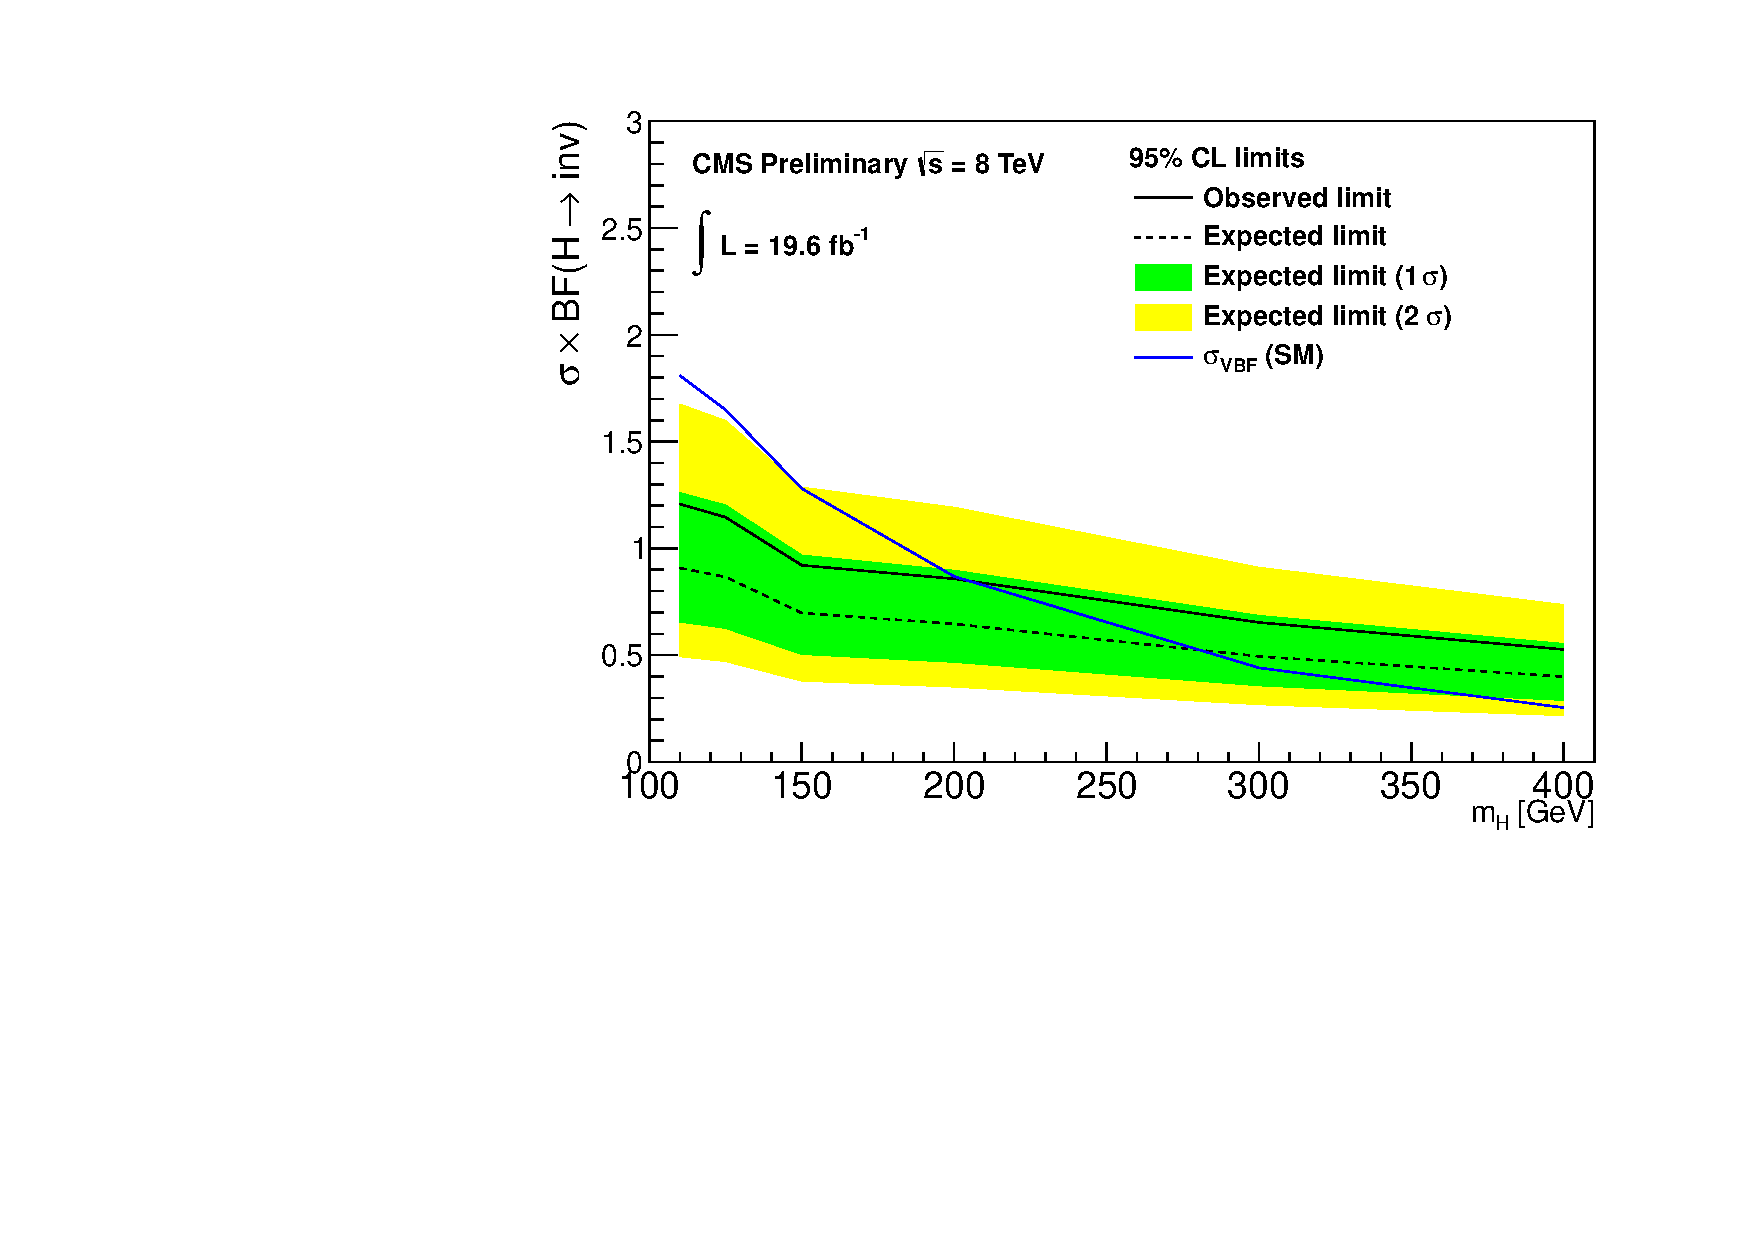
\includegraphics[width=.95\textwidth,trim=0 0 0 0]{Pictures/XSLimit.pdf}

           \begin{itemize}
           \item We predict $339 \pm 36$ (stat.)$\pm 50$ (syst.) events and we observe 390:
           \item[-] this corresponds to a 69\% limit on BF(inv) for a 125 GeV Higgs boson at 95\% C.L.
           \end{itemize}

         \end{block}

         \begin{block}{\LARGE Conclusion and future work}
           \vspace{.5cm}
           \begin{itemize}
           \item First ever limit on invisible branching fraction of VBF produced Higgs boson:
           \item[-] compatible with the standard model.
             \vspace{.2cm} 
           \item We have additional 'parked' data with lower trigger thresholds that is yet to be analysed:
           \item[-] this should give more events in our control regions and thus reduce the errors on our background estimation.
             \vspace{.2cm}
           \end{itemize}
             \vspace{.2cm}
         \end{block}


     %\vspace{.5cm}

         \begin{block}{}
           \begin{itemize}
             \vspace{.3cm}
           \item I would like to thank my supervisors David Colling and Gavin Davies and the members of my analysis group, particularly Anne-Marie Magnan and Andrew Gilbert, for the help they have given me, and the STFC for funding my work.
           \item More information can be found in CMS PAS HIG-13-013.
           \end{itemize}
           \vspace{.3cm}
         \end{block}
         
       \end{minipage}
       
    \end{columns}

      %\end{minipage}
    %\end{columns}
  \end{frame}
  
\end{fmffile}
\end{document}
